%\documentclass[12pt]{spieman}  % 12pt font required by SPIE;
%% experimental start
%% \setkeys{Gin}{draft=false} # turn off graphics
%% experimental end
\documentclass[a4paper,12pt]{spieman}  % use this instead for A4 paper
\usepackage{amsmath,amsfonts,amssymb}
\usepackage{graphicx}
\usepackage{setspace}
\usepackage{tocloft}
%\definecolor{nbsphinxin}{HTML}{303F9F}
\usepackage{xspace}
%\usepackage{multirow}
% \usepackage[table,xcdraw]{xcolor}
% \usepackage{caption}
% \usepackage{subcaption}
% %\usepackage{natbib}
% % kire bhai kemun achish? Call ee naki? Link paste kor ekhane!!
% \usepackage{lineno}
% % \usepackage{cite} 
% % \usepackage[square,sort]{natbib}
% \usepackage[numbers,super]{natbib}
% % \bibliography{report.bib}
% \usepackage[utf8]{inputenc}
% \usepackage[english]{babel}

%Import the natbib package and sets a bibliography  and citation styles
% \usepackage{natbib}


% \author{Overleaf team}


% \bibpunct[, ]{(}{)}{;}{a}{}{,}% Citation support using natbib.sty
%\renewcommand\bibfont{\fontsize{10}{12}\selectfont}% Bibliography support using natbib.sty
% \linenumbers

\title{DNN-PolSAR: Urban Image Segmentation and Classification using Polarimetric SAR based on DNNs}

\author[a]{Soumyadip Sarkar}
\author[a]{Farhan Hai Khan}
\author[a]{Sayanti Dutta}
\author[b]{Raisa Chatterjee}
\author[c]{Tripti Kumari}
\author[a]{Deeptendu Santra}
\author[a]{Nirmalya Misra}
\author[a]{AritroPal Choudhury}
\author[a]{Shobhit Kumar} 
\author[d]{Tamesh Halder}
\author[e]{Dipjyoti Paul} 
\author[f]{Sajal Sarkar}
\author[a]{Rintu Kumar Gayen}
\author[g]{Arundhati Misra Ray}
\author[d]{Debashish Chakravarty}

\affil[a]{Institute of Engineering \& Management, Kolkata, India, 700091}
\affil[b]{Department of CSE, Jadavpur University, India, 700032}
\affil[c]{Department of CSE, Indian Institute of Information Technology (IIIT), Ranchi, Jharkhand, India -834010}
\affil[d]{Department of Mining Engineering, Indian Institute of Technology, Kharagpur, India, 721302}
\affil[e]{Office H304, Department of Computer Science, University of Crete, Heraklion, Crete 70013}
\affil[f]{Information Security Dept., Power Grid Corporation of India Ltd, Gurgaon, India, 122001}
\affil[g]{Space Application Center, ISRO, India, 380015}

\renewcommand{\cftdotsep}{\cftnodots}
\cftpagenumbersoff{figure}
\cftpagenumbersoff{table}
\begin{document}
\maketitle
% \biboptions{sort&compress}

% \bibliographystyle{abbrvnat}
% \setcitestyle{authoryear,open={((},close={))}} %Citation-related commands
% \title{Natbib Example}
\begin{abstract}
Synthetic Aperture Radar (SAR) image segmentation and classification is a popular technique for learning and detection of objects such as buildings, trees, monuments, crops water-bodies, hills, etc. SAR technique is being used for urban development and city-planning, building control of municipal objects, searching best locations, detection of changes in the existing systems, etc. using polarimetry based on Deep Neural Networks. In this paper, we proposed a technique for Urban Image Segmentation and Classification using Polarimetric SAR based on Deep Neural Networks (DNN-PolSAR). In our proposed DNN-PolSAR technique, we use Mask-RCNN, LinkNet, FPN, and PSPNet as model architectures, whereas ResNet50, ResNet101, ResNet152, and VGG-19 are used as backbone networks. We, first, apply polarimetric decomposition on airborne Uninhabited Aerial Vehicle Synthetic Aperture (UAVSAR) images of urban areas and then the decomposed images are fed to DNNs for segmentation and classification. We then simulate DNN-PolSAR considering different hyper-parameters and compare the obtained scores of hyper-parameters against used model architectures and backbone networks. In comparison, it is found that DNN-PolSAR based on FPN model with ResNet152 performed the best for segmentation and classification. The mean Average Precision (mAP) score of the DNN-PolSAR based on FPN with a pixel accuracy of 90.9\% is 0.823, which outperforms \emph{other Deep Learning models}. 
\end{abstract}
\keywords{Polarimetric SAR, FPN, PSPNet, Mask-RCNN, LinkNet, Image Segmentation}
% \tableofcontents
% \listoffigures
% \listoftables
% Include email contact information for corresponding author
\begin{spacing}{1}   % use double spacing for rest of manuscript
\section{Introduction}
\label{sect:intro}  % \label{} allows reference to this section
Segmentation and classification of an image is a process of splitting and categorizing the image into different parts based on the predefined category of objects. In this process, each pixel in an image is categorized based on the predefined labels of objects. Image segmentation has historically been used primarily for recognizing scenes in which similar objects can be placed more accurately. However, recently image segmentation is being used in different fields such as medical imaging, autonomous driving, etc. very successfully. Therefore, image segmentation can also be used for satellite image and Polarimetric Synthetic Aperture Radar (PolSAR) of urban cover areas for categorization and analysis \cite{niu2012context, taghanaki2021deep}.
PolSAR is a very popular technique in remote sensing and it is being used in wide ranges of applications namely segregation and classification in GIS, remote sensing, etc. It is also used for mapping of areas such as forest, vegetation, urbanized areas, etc. Data generated from PolSAR provides SAR resolutions, which help to understand images in forms of scattering components such as surface scattering, volume scattering, helix scattering, double-bounce scattering, and wire scattering. Based on these scattering components, PolSAR helps to understand classification of objects. For example,  it is seen that PolSAR generates more prominent helix and double-bounce scattering components for images of urban areas  \cite{zhou2018multi, chen2018polsar, zhang2015land}. Hence, here in this work, we consider double-bounce scattering and helix scattering components for classification of objects in images of urban areas.
With growth of urbanization and increasing population in urban areas, tracking, studying and analysis of the urban cover areas have become very essential, particularly in terms of locating and classifying objects such as buildings, crops water-bodies and hills. So, accurate locating and classification of different objects using images of urban areas is important for designing quick and reliable solutions \cite{de2017novel}. However, urban image segmentation and classification is a very challenging task even using SAR polarimetry. Hence, it is more challenging task to segment and classify images of urban cover areas. This is because urban cover relatively shows small part of total surface. Fortunately, a huge collections of satellite imagery datasets is available freely which can be used for image segmentation and classification of urban cover areas.
Image segmentation and classification of urban cover areas using PolSAR is very difficult task due to urban structures, whose orientation is not in line of sight (LoS) of the radar. However, recognition of such areas is important for a number of reasons such as disaster relief, urban planning, and environmental monitoring. But, it is not possible to feed the scattering of images of urban covers areas taken using the Uninhabited Aerial Vehicle Synthetic Aperture Radar (UAVSAR) into a neural network. This is because it is required to employ a set of decompositions of images in order to retrieve various information using scattering such as surface scattering, double bounce scattering, volume scattering, helix scattering, wire scattering, etc. It is also required to identify different areas such as grassland, urban areas, hills, etc.  with different scattering information and components from the images, so the data obtained from scattering become significant. A scattering component allows us to determine what kind of area is captured in particular images. A grassland, for example, may have high values for surface scattering, while an urban area may have high values for both double bounce and helix scattering.
With the application of these decomposition techniques to the UAVSAR raw scattering matrix elements, different areas tend to exhibit different characteristics, which can be used to perform image segmentation and classification. Based on the above mentioned principle, in this paper, we present a technique for Polarimetric SAR (PolSAR) image segmentation and classification of Radar Satellite Imagery of urban areas using Deep Neural Networks (DNNs) such as SPNet, LinkNet, FPN, and Mask-RCNN based on different backbone networks such as such as EffcientNet, DenseNet, MobileNet, Inception, ResNet, and VGG19 (discussed in Subsection \ref{BNs}). In our proposed technique, we first apply polarimetric decomposition on airborne Uninhabited Aerial Vehicle Synthetic Aperture (UAVSAR) images of urban areas and then the decomposed images are fed to DNNs for segmentation and classification. We simulate our proposed technique and accordingly obtain simulation results using different DNNs.
 The major contribution of this work are as follows:
\begin{itemize}
    \item We introduce new architectures consisting of models and backbone networks for urban classification and perform rigorous evaluation of all the machine learning classifiers in the field of Remote Sensing. We propose a technique to identify and detect buildings, grassland, hills from the PolSAR images.
    \item Presented and described the best and most effective Deep Learning methods for PolSAR image segmentation and classification.
    \item We obtain simulation results of our proposed technique with different backbone networks such as EffcientNet, DenseNet, MobileNet, Inception, ResNet, and VGG19.
    \item We carried out an extensive comparison of the current state-of-the-art models on the same datasets for segmentation and classifications of urban area covers.
\end{itemize}
The reminder of the paper is organized as follows. Section 2 presents Related Work in the area of satellite image segmentation and classification. In Section 3, we discuss the architectures and backbones of the models, which are used in four different experimentation presented in our paper. An overview of the datasets used for training and validation is discussed in Section 4. In Section 5, results of experimentation based on different databases and discussion on the results are presented. Finally, we concluded our paper in Section 6.
\section{Related Works}
Segmentation of PolSAR images of urban cover areas poses unique challenges such as partial visibility of surfaces, different scattering, etc. However, only good thing is that area structure of the these images are well defined. But, design and development of algorithms for analysis and classifications of such as images requires focused research for opening possibilities for the application of Remote Sensing in various fields. In view of this, A numbers of works have been proposed for image analysis and classification using semantic segmentation. In this section, we briefly present and discuss some of the advancements in classification approaches for PolSAR as well some of the examples where architectures from a different area of study has been successfully applied in remote sensing.
A recent study conducted by De et al\cite{8068203} to build a Deep Learning based novel technique for classification of urban areas. The information in the augmented dataset used in this work is transformed using a stacked auto-encoder, before feeding it to a neural network for classification. This technique achieved an accuracy of 91.3\%, which was an enhancement in performance as compared to the techniques present at that time. In \cite{8763918}, Cui et al proposed an architecture comprising Dense Attention Pyramid Network (DAPN), Region Proposal Network (RPN) and a detection network for multi-scale ship detection in SAR images. Here, DAPN was used to extract multi-scale fused features for generating and detecting to  use in the subsequent iterations of the technique. The top-down densely connected networks are used to get concatenated feature maps of lower layers. The proposed method provided an accuracy of 89.8\%, which was 11\% higher than the previous models on the SAR ship detection data set (SSSD). DAPN was also 20\% more than the faster R-CNN\cite{ren2015faster}. They also show that the top-down pyramid structure with attention is very effective in obtaining the feature maps which contained more spatial and semantic information.
Recently, Mohanty et al presented applications of Mask-RCNN \cite{mrccnbuildling} on the segmentation and detection of building on Google Maps Satellite Imagery Data. Authors found the results to be impressive with a fina loss value of 0.15 for the instance image segmentation model. A research Wang et al. explored the problems in the classification of PolSAR images due to the presence of nonlinear data \cite{wang2018polarimetric}. This study proposed a kernel sparse representation based classification approach. This kernel function technique solves the problems caused by the nonlinear features. This helps in attaining more accurate results in the task of classification. This study used an Airborne SAR dataset from San Francisco, United States of America.
In \cite{femin2020accurate}, Femin et. al. proposed an approach for detecting buildings using CNNs from satellite images. In this work, different building footprints from the images were identified using CNN method. The proposed work was also detected different shapes and colors. The detection accuracy by this approach for building was found to be 83\%. On the other hand, Wang et al. introduced a deep feature extraction approach \cite{PAOPTDCNN}, where multilevel polarimetric feature vector is extracted using a PAO\_PTD\_CNN. The authors extracted superpixels using simple linear iterative clustering (SLIC) from the feature vector for classification map. Finally, the result is obtained combining the superpixel map and the deep feature classification vector with Kappa Score of 0.86.
The authors of \cite{Ding_2021} mentioned that the semantic segmentation can also be implemented for high-resolution PolSAR images using neural network architecture such as MP-ResNET which contains three concurrent semantic embedding branches and uses a multi-scale feature fusion design in decoder to use each encoding branch. The authors noticed that MP-ResNet improves the aggregation of context information compared to baseline Fully Convolution Network (FCN). The suggested method based on MP-ResNet surpasses numerous state-of-the-art methods in all accuracy with a mean F1 of 92.25\% and IoU of 89.60\% in classification using the Gaofen Dataset. Zhao et. al. showed in \cite{zhao2013segmentation} that segmentation can also be achieved using edge information based on spectral graph partitioning. Here, the authors defined segmentation as a three-part process namely edge information extraction, edge-based similarity matrix analysis, and Normalised Cut. This method overcame the pepper-salt phenomenon along with much more complete and the boundaries of the segments. The method of \cite{ouahabi2021deep} by Ouahabi et. al. aimed to improve the segmentation efficiency without compromising the accuracy using Fully Convolution dense Dilated Network model. Here, the authors found that the Low resolution and contrast, shadow interference as well as differences in size and position of the abnormal tissue are the challenges that hinder the process of obtaining the segmentation of ultrasound images. Yuanyuan et al. in his work \cite{rs61212575} explores how different classification algorithms are affected by the choice of polarimetric parameters such as Alpha, HAAlpha\_T11, Shannon entropy, VanZyl3\_Vol, Neuman\_delta\_mod, Barnes2\_T33, Barnes1\_T33, and entropy. \section{Backbone Network and Model Architecture}
\subsection{Backbone Networks}
\label{BNs}
A backbone network is mainly used to extract network feature for classification of objects. Here, in this paper we have used ResNet152\cite{he2016deep}, ResNet101\cite{Xie2016}, ResNet50, and VGG-19\cite{simonyan2014very} backbone networks for features extraction.
\subsection{Model Architectures}
In this Subsection, we explain model architectures such as M-RCNN, PSPNet, FPN, and LinkNet used for classification in our work. The model architectures classify the extracted features using the base model from the deep neural backbone networks discussed in \ref{BNs}.
\subsubsection{MR-CNN}
The M-RCNN \cite{7900179} was developed as an extension to the Faster-RCNN \cite{ren2015faster} which has been widely used so far for various object detection purposes. The F-RCNN/M-RCNN as output yields an object’s label along with the object’s bounding box. F-RCNN uses a feature extractor block that extracts the features from the image. These features are then used to train the bounding box regressor and the classifier. The Mask RCNN as the name suggests extends F-RCNN by training a binary mask in parallel with the bounding box regressor and object classifier.
The first stage of the Mask-RCNN (like the F-RCNN) is the Region Proposal Network (RPN). Each bounding box is paired with an objectness score that denotes the probability score of the object. The second stage of the M-RCNN is called the head of the network. In F-RCNN this head is generally a stack of convolution layers and a dense layer for bounding box regression. M-RCNN in parallel to this bounding box learning algorithm uses a stack of convolution layers for Mask representation. This parallel task makes it theoretically faster and more accurate than other segmentation models.
\subsubsection{Feature Pyramid Network (FPN)}
A FPN is a fully convolutional feature extractor that takes a single-scale image of any size as input and produces correspondingly sized feature maps at several layers \cite{lin2017feature}. The model comprises two distinctive parts  such as  a conventional convolutional network (like VGG-19 or ResNet50) that acts as a feature extractor and a deconvolutional network with compatible feature sizes. However, there is a crucial difference between these two parts: the convolutional network goes from bottom to top whereas the flow in the deconvolutional network goes from top to down. The blocks in the convolutional network are connected in the deconvolutional network by linear multiplication. The output of blocks in the deconvolutional layer are connected to individual convolution layers which are not directly connected. These layers are transformed into a stack of layers. This dataset undergoes some upsampling and activation to give us an image map.
\subsubsection{LinkNet}
The LinkNet is a lightweight network architecture designed for performing segmentation tasks with a special focus on processing time \cite{chaurasia2017linknet}. Instead of a typical auto-encoder style segmentation model where the spatial semantics are first extracted using encoder blocks and then the decoder uses this spatial information for spatial categorization. This method has a certain downside in terms of both computation and accuracy. The pooling and strided convolution used in encoders may result in some loss of spatial information. So instead, the LinkNet algorithm uses skip connections from one encoder block to the corresponding block to prevent the loss of information at each stage. This idea of semantic information preservation is very similar to an U-Net except in this case the results of the encoder are added to the results of the corresponding decoder block instead of performing feature concatenation.
For experimentation, we will be using the model proposed in the original LinkNet paper. The model uses four encoder blocks and four corresponding decoder blocks. There are two special blocks of fully convolutional neural networks at the beginning and end of the network to preserve the dimensions of the image.
\subsubsection{Pyramid Scene Parsing Network (PSPNet)}
The PSPNet of \cite{zhao2017pyramid} is a model used for semantic segmentation. Its specialty is that it uses a pyramid parsing module. Different region-based context aggregation is used by this module to exploit global context information. The final predictions are made more reliable due to the presence of local and global clues together. Given an input image, the feature map can be extracted using a pre-trained CNN, using a dilated network strategy. The final size of the feature map is reduced to 1/8th of the input image. A pyramid pooling module is then applied on the top of the map, for gathering context information. A four-level pyramid is used where the pooling kernels cover the whole, half of, and small parts of the image. The results from the pooling kernels are then concatenated to form a global prior. In the next step this prior is concatenated to the original feature map. The obtained result is finally passed through a stack of convolutional layers to generate the final prediction.
\bgroup
\def\arraystretch{1.5}%
\begin{table}[h!]
\caption{Decomposition Method and Polarimetric Parameter}
\begin{tabular}{|l|lll|}
\hline
Decomposition Method & \multicolumn{3}{c|}{Polarimetric Parameter}\\ \hline
Cloude\cite{485127} & Cloude\_T11         & Cloude\_T22         & Cloude\_T33       \\ \hline
\multirow{H/A/Alpha\cite{pottier2000application}}            & Entropy             & Anisotropy          & Shannon Entropy\\
                                      & H/A/A\_T11          & H/A/A\_T22          & H/A/A\_T33        \\ \hline
VanZyl3\cite{pottier2000application}                               & VanZyl3\_Vol        & VanZyl3\_Odd        & VanZyl3\_Dbl      \\ \hline
Neuman\cite{neumann2009general}                                & Neuman\_delta\_mod  & Neuman\_delta\_pha  & Neuman\_tau       \\ \hline

FreeMan2\cite{4276884}              & FreeMan2\_Vol       & FreeMan2\_Ground    &                   \\ \hline
FreeMan\cite{673687}                 & FreeMan\_Vol        & FreeMan\_Odd        & Freeman\_Dbl      \\ \hline
Huyen\cite{huynen1990stokes}         & Huyen\_T11          & Huyen\_T22          & Huyen\_T33        \\ \hline
Bhattacharya\cite{bhattacharya2015modifying}              & Frey\_Dbl           & Frey\_Hlx           & Frey\_Odd         \\ \hline
Singh\cite{singh2018model}                                 & Singh\_6SD1         & Singh\_G4U2\_Vol    & Singh\_G4U2\_Odd  \\ \hline
Barnes1\cite{barnes1988roll}          & Barnes1\_T11        & Barnes1\_T22        & Barnes2\_T33      \\ \hline
Barnes2\cite{barnes1988roll}         & Barnes2\_T11        & Barnes2\_T22        & Barnes2\_T33      \\ \hline
Pauli\cite{485127}                                 & Pauli\_a            & Pauli\_b            & Pauli\_c          \\ \hline
Holm1\cite{holm1988radar}           & Holm1\_T11          & Holm1\_T22          & Holm1\_T33        \\ \hline
Holm2\cite{holm1988radar}                                 & Holm2\_T11          & Holm2\_T22          & Holm2\_T33        \\ \hline
Arri3\_NNED\cite{5659970}           & Arii\_NNED\_Vol     & Arii\_NNED\_Odd     & Arii\_NNED\_Dbl   \\ \hline
An\_Yang3\cite{5437202}             & An\_Yang3\_Vol      & An\_Yang3\_Odd      & An\_Yang3\_Dbl    \\ \hline
An\_Yang4\cite{5872006}                             & An\_Yang4\_Vol      & An\_Yang4\_Odd      & An\_Yang4\_Dbl    \\ \hline
Yamaguchi3\cite{yamaguchi2013comparison}                      & Yamaguchi3\_Vol     & Yamaguchi3\_Odd     & Yamaguchi3\_Dbl   \\ \hline
Yamaguchi4\cite{1487628}                            & Yamaguchi3\_Vol     & Yamaguchi3\_Odd     & Yamaguchi3\_Dbl   \\ \hline
\end{tabular}
\label{decomp}
\end{table}
\egroup
\section{Datasets}
Datasets play an important and crucial role in any machine learning algorithms for segmentation and classification. In our proposed technique too datasets play major roles in segmentation of classification of images of urban cover areas. We have mentioned in Section 1 that a huge collections of
satellite imagery datasets is available for image segmentation and classification of urban cover areas. Therefore, in order to train our proposed algorithm, we have used PolSAR images of Lancaster, Palmdale and Rosamond city from airborne UAVSAR. However, we have considered only building classes for semantic and instance segmentation from these datasets using Deep Learning over various polarimetric decompositions. It is also to be mentioned that as similar of \cite{rs61212575}, we have used different polarization parameters such as Alpha, HAAlpha\_T11, Shannon entropy, VanZyl3\_Vol, Neuman\_delta\_mod, Barnes2\_T33, Barnes1\_T33, and entropy to improve the classification accuracy of our proposed technique. We use PolSARPro v6.0 Software Suite \cite{pottier2019polsarpro} for decomposition results in our proposed work. In Table \ref{decomp}, we shows all the decomposition methods and corresponding polarimetric parameters thoes were applied on the datasets with our proposed technique.
It is required to be mentioned that we also performed image augmentation using random rotation and image flipping to generate more data before passing them through the model. We generated $3$ transformed images from each image with image size of $1331 \times 1101 \times 3$ for enhancing our datasets. The enhanced datasets are used for training based on PolSAR images of Lancaster, Palmdale, and Rosamond cities of USA. The reason of usage of datasets from different cities for increasing segmentation accuracy by introducing variance in the datasets. Detail of used datasets are given in Table \ref{dataset-table}. It can be seen from Table \ref{dataset-table} that there are 71, 60, and 50 training datasets for Lancaster, Palmdale, and Rosamond respectively. But, we used 33, 64, and 17 test datasets for Lancaster, Palmdale, and Rosamond respectively.
\begin{figure}[t!]
\centering
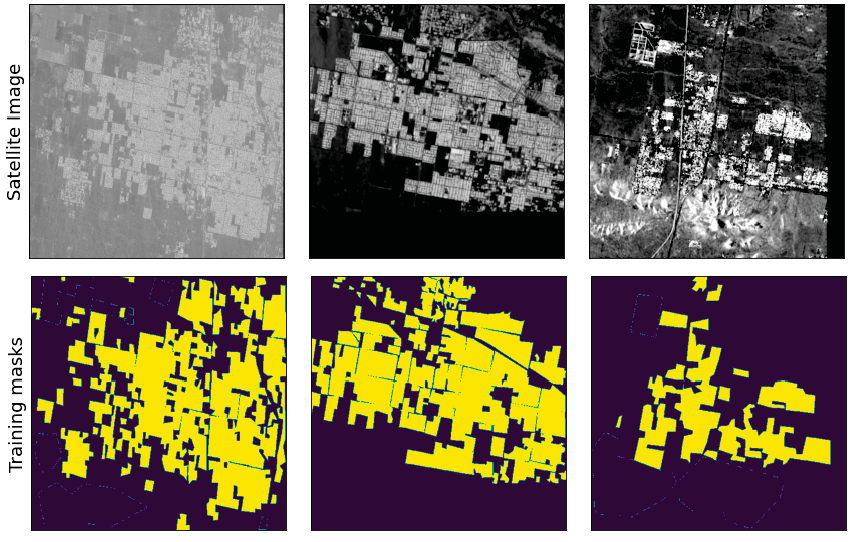
\includegraphics[width=\textwidth]{data and mask.PNG}
\caption{\label{fig:dataset-sample}Sample Datasets and their Corresponding Masks for Urban Areas.}
\end{figure}
\begin{table}[]
% \captionsetup{justification=centering, margin=2cm}
\caption{Description of the Datasets}
\begin{tabular}{|c|c|c|c|c|c|}
\hline
\multirow{Location} & \multicolumn{2}{c|}{Coordinates} & \multirow{Region/Country} & \multicolumn{2}{c|}{Datasets} \\ \cline{2-3} \cline{5-6}
                          & Latitude       & Longitude       &                                 & Train         & Test         \\ \hline
Lancaster                 & 40.037° N      & 76.305° W       & Pennsylvania, USA               & 71            & 33           \\ \hline
Rosamond                  & 34.8641° N     & 118.1634°  W    & Karen County, California, USA   & 60            & 64           \\ \hline
Palmdale                  & 34.3452° N     & 118.62°  W      & Los Angeles, California, USA    & 50            & 17           \\ \hline
\end{tabular}
\label{dataset-table}
\end{table}
Figure \ref{fig:dataset-sample} shows sample datasets of satellite images (upper of parts of the Figure) as well as corresponding masks (the lower parts of the Figure) of the satellite images. From Figure \ref{fig:dataset-sample}, it can be seen that our proposed technique based on used datasets correctly segmented and classified urban areas from the images. In the lower parts of the Figure \ref{fig:dataset-sample}, the yellow color masks represent the presence of urban areas for the given satellite images. Details of results with our proposed technique and discussion on the results are given in the following Section \ref{RD}.
\section{Proposed Technique}
Proposed technique to be discussed providing a block diagram of all important steps. The block diagram of out proposed scheme is shown in Figure \ref{BlockD}.
\begin{figure}[h!]
\centering
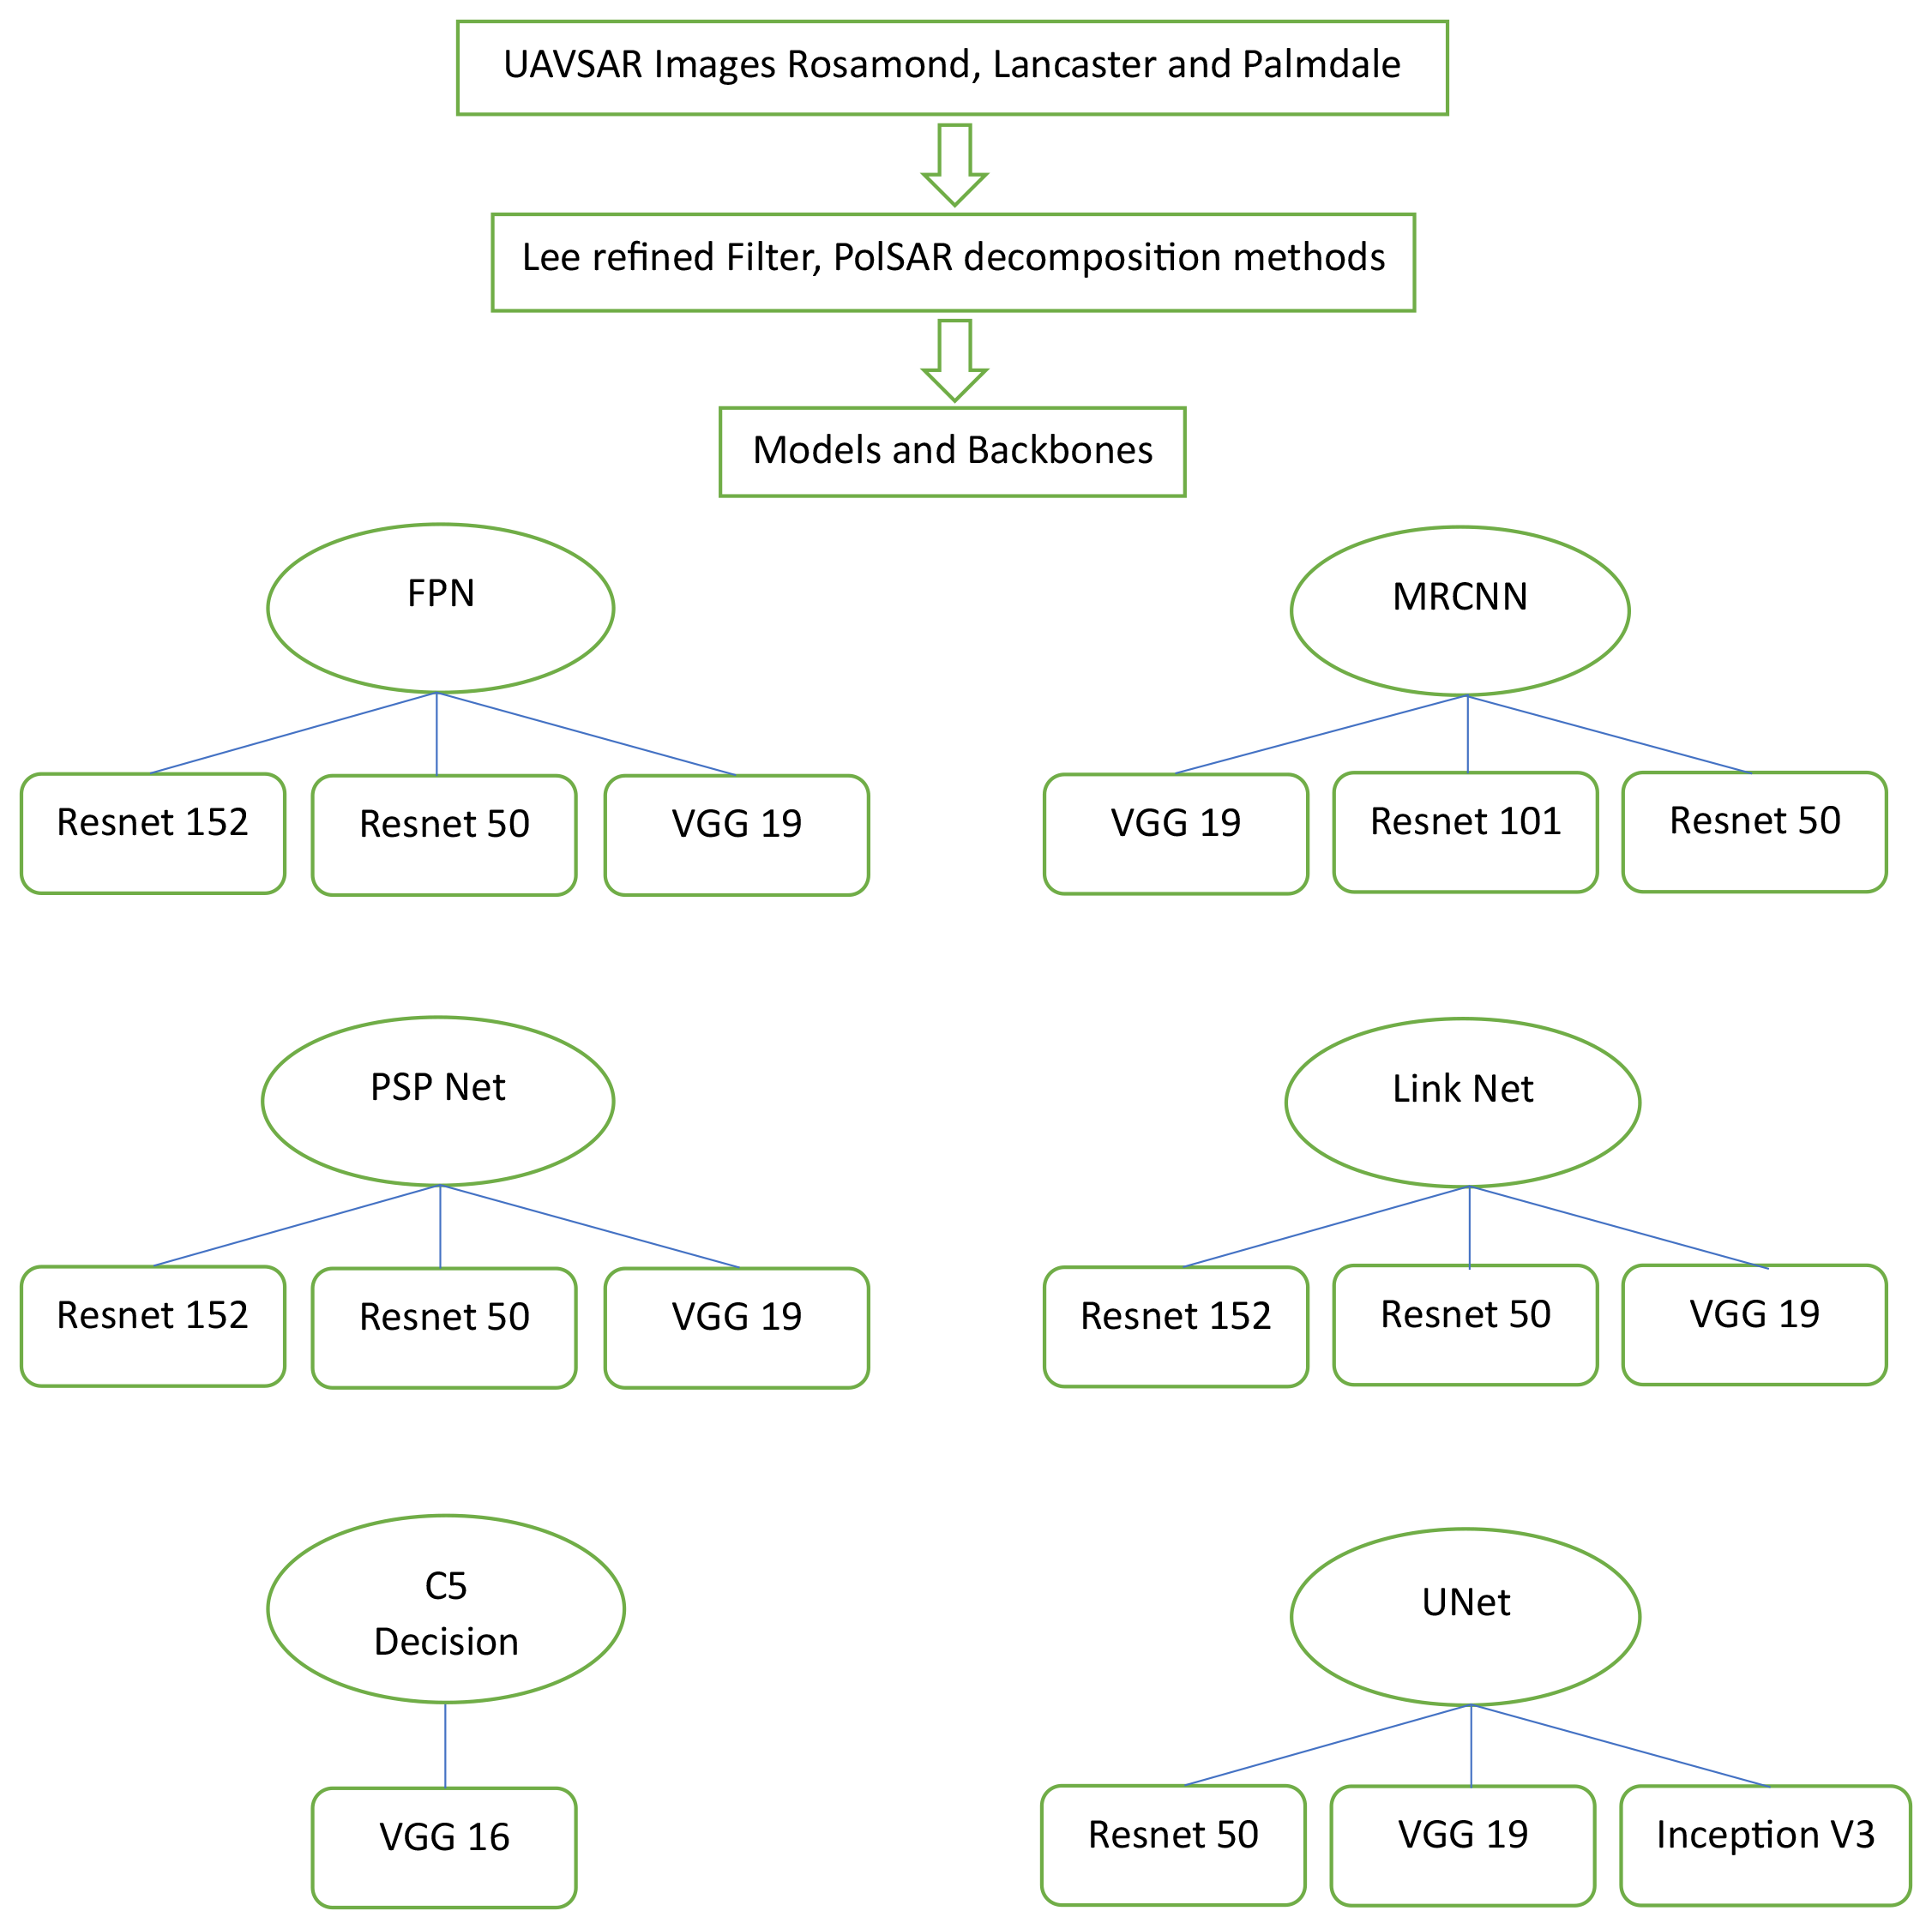
\includegraphics[width=4.5in, height=4.5in]{methodology.png} %Block diagram to be added here
\caption{Block Diagram of Our Proposed Scheme}
\label{BlockD}
\end{figure}
\section{Simulation Studies}
In this Section, we have presented simulation of our proposed technique and discussed on obtained results. It is to be mentioned that the main motivation of our work is to understand the learning capacity and rate of convergence against the above mentioned architectures with different backbone networks. In order to do that we have considered four different architectures as well as four different backbone networks to obtain unbiased results. We have used \emph{Intersection Over Union (IoU) score}, \emph{Pixel Accuracy}, \emph{F1 Score}, \emph{Cohen's Kappa Score}, \emph{Area Under the Curve}, \emph{Recall}, \emph{Precision}, and \emph{Mean Average Precision(mAP)} hyper-parameters as performance metrics to obtain simulation results. We have also discussed these metrics to draw performance comparison of different architectures and backbone networks.
\subsection{Simulation Environment}
We have simulated our proposed technique using (Python3 on a Kaggle, Colab notebook and R language in a computer with 64 GB RAM. Simulated the proposed technique is conducted using model architectures namely MR-CNN, FPN, LinkNet, PSPNet, C5 decision tree and Unet against the ResNet152, ResNet101, ResNet50, Inception V3, VGG16 and VGG-19 backbones networks. However, we provided results of best performing backbone networks for each considered model architectures.
\bgroup
\def\arraystretch{1.1}%
\begin{table}[]
\centering
\caption{Pixel Accuracy, Cohen's Kappa Score, and IoU Score of all Considered Model Architectures and Backbone Networks}
\label{tab:results1}
\begin{tabular}{|c|c|c|c|c|}
\hline
\textbf{Model Architecture} &
  \textbf{Backbone Network} &
  \textbf{Pixel Accuracy} &
  \textbf{\begin{tabular}[c]{@{}c@{}} Cohen's Kappa \\ Score\end{tabular}} &
  \textbf{IoU Score} \\ \hline
                                  & \textbf{ResNet152}  & 0.909          & \textbf{0.806} & \textbf{0.799} \\ \cline{2-5}
                                   & \textbf{ResNet50}   & 0.901          & 0.786          & 0.774  \\ \cline{2-5}
\multirow{\textbf{FPN}} & \textbf{VGG-19}     & 0.909          & 0.805          & 0.796                   \\ \hline
                                  & \textbf{ResNet101} & 0.897          & 0.781          & 0.780          \\ \cline{2-5}
                                  & \textbf{ResNet50}   & 0.638          & 0.057          & 0.069                  \\ \cline{2-5}
\multirow{\textbf{MR-CNN}}  & \textbf{VGG-19}     & 0.811          & 0.621          & 0.667 \\ \hline
                                  & \textbf{ResNet152}  & 0.885          & 0.755          & 0.753                    \\ \cline{2-5}
                                  & \textbf{ResNet50}   & 0.895          & 0.771          & 0.758          \\ \cline{2-5}
\multirow{\textbf{PSPNet}} & \textbf{VGG-19}     & 0.893          & 0.772          & 0.763\\\hline
{\color[HTML]{222222}}           & \textbf{ResNet152}  & \textbf{0.910} & 0.805          & 0.791\\\cline{2-5}
{\color[HTML]{222222}}           &   \textbf{ResNet50} &   0.464 &   0.127 &   0.419          \\ \cline{2-5}
\multirow{{\color[HTML]{222222} \textbf{LinkNet}}} & \textbf{VGG-19}     & 0.715          & 0.461  & 0.573 \\\hline
\multirow{\textbf{Unet}} & \textbf{VGG-19}  & \textbf{0.918}          & 0.54          & 0.48                   \\ \cline{2-5}
                                  & \textbf{InceptionV3} & 0.815          & 0.03          & 0.12          \\ \cline{2-5}
                                  & \textbf{ResNet50}   & 0.947          & 0.54          & 0.67                 \\\hline
\multirow{\textbf{C5}} & \textbf{VGG-16}     & 0.717          & 0.39          & 0.44                   \\ \cline{2-5}
\hline
\end{tabular}
\end{table}
\egroup
\bgroup
\def\arraystretch{1.1}%
\begin{table}[]
\centering
\caption{mAP, AuC, Recall, Precision, and F1 score all Considered Model Architectures and Backbone Networks}
\label{tab:results2}
\begin{tabular}{|c|c|c|c|c|c|c|}
\hline
\textbf{Model Architecture} &
  \textbf{Backbone Network} &
  \textbf{mAP} &
  \textbf{AuC} &
  \textbf{Recall} &
  \textbf{Precision} &
  \textbf{F1 Score} \\ \hline
                          & \textbf{ResNet152} & \textbf{0.823} & 0.965 & 0.917 & 0.850  & 0.882\\ \cline{2-7}
                          & \textbf{ResNet50}   & 0.808          & 0.963 & 0.879 & 0.861  & 0.870\\ \cline{2-7}
\multirow{\textbf{FPN}}   & \textbf{VGG-19} & 0.817 & \textbf{0.968} & 0.928 & 0.843 & \textbf{0.884}\\ \hline
                          & \textbf{ResNet101} & 0.809 & 0.950 & 0.897 & 0.839  & 0.867 \\ \cline{2-7}
                           & \textbf{ResNet50}   & 0.394 & 0.634 & 0.075 & 0.647 & 0.134\\ \cline{2-7}
\multirow{\textbf{MR-CNN}} & \textbf{VGG-19}     & 0.672          & 0.937 & 0.973 & 0.671 & 0.794\\ \hline
                           & \textbf{ResNet152} &   0.768 &   0.960 &   0.934 &   0.795 & 0.859 \\ \cline{2-7}
                           & \textbf{ResNet50}   & 0.784          & 0.961 & 0.896 & 0.835  & 0.865 \\ \cline{2-7}
\multirow{\textbf{PSPNet}} & \textbf{VGG-19}     & 0.788          & 0.957 & 0.907 & 0.824    & 0.864\\ \hline
{\color[HTML]{222222} }    & \textbf{ResNet152}  & 0.822 & 0.966 & 0.895 & \textbf{0.868} & 0.881  \\ \cline{2-7}
{\color[HTML]{222222} }    & \textbf{ResNet50} &   0.419 &   0.618 & \textbf{1.000} &   0.411 &   0.583 \\ \cline{2-7}
\multirow{{\color[HTML]{222222} \textbf{LinkNet}}} & \textbf{VGG-19}     & 0.579 & 0.890 & 0.968 & 0.570 & 0.718 \\ \hline
\end{tabular}
\label{tab:results2}
\end{table}
\egroup
\subsection{Results and Discussion}
\label{RD}
In Table \ref{tab:results1}, we presented simulation results of Pixel Accuracy, Cohen's Kappa Score, and IoU Score hyper-parameters for all the considered model architectures and backbone networks. The Unet and C5 based our old work also compared here \cite{Halder1}. On the other hand Table \ref{tab:results2} presents simulation results of Mean Average Precision, Area Under the Curve, Recall, Precision, and F1 Score hyper-parameters for all the considered model architectures and backbone networks.
From Table \ref{tab:results1}, it can be seen that Cohen’s Kappa Score and IoU Score for FPN with ResNet152 is highest compared to all other scores. Similarly, Table \ref{tab:results2} shows that mAP, AuC and F1 Scores for FPN with ResNet152 and VCG19 are highest respectively. Therefore, it may be concluded that the FPN gives the best accuracy among all models proposed in this paper. The high F1 score and AuC scores for the top three models confirm that the FPN architecture performs best among all other architectures. It gives pixel accuracy above 90\% for three backbones, namely ResNet152, VGG-19, and ResNet50.
On the other hand, it can be seen from Table \ref{tab:results1} that the Pixel Accuracy of 91\% for LinkNet with ResNet152 is highest. But Table \ref{tab:results2} shows that the values of Recall and Precision are highest for LinkNet with ResNet50 and ResNet152 respectively.
The pixel accuracy, cohen's kappa, IoU score, AuC, Recall Precision, and F1 Score of MR-CNN with ResNet101 is better compared to other backbone networks. Based on these values of parameters, it can be inferred that the MR-CNN model architecture is the largest model used here in terms of the number of trainable parameters and consequently this architecture takes more time to train the system considering all used images than other considered model architectures.
Finally, the Pixel Accuracy with ResNet50 and Cohen’s Kappa Score and IoU Score with VGG19 for PSPNet are better compared to other two backbone networks. The values of AuC with ResNet50,  Recall with ResNet152 Precision and F1 Score with ResNet50 are best. It can specifically be inferred about PSPNet that the PSPNet architecture performs well with VGG-19, ResNet50 and ResNet152 respectively as its backbone networks. The UNet and C5 decision trees results can be found at \citep{Halder1} which have lower performance than FPN.
\begin{figure}[!htbp]
	\centering
	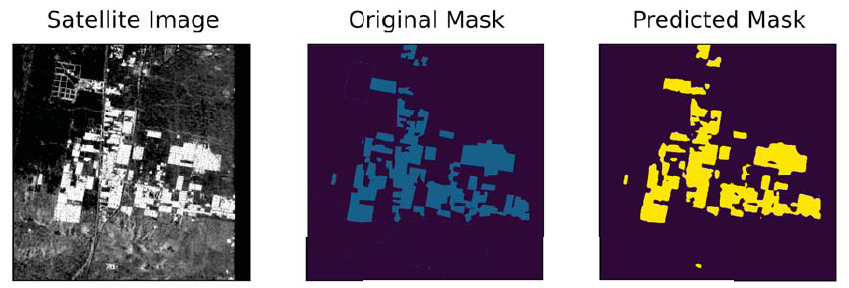
\includegraphics[width=\textwidth]{fpn.png}
 	\includegraphics[width=\textwidth]{fpn-resnet152.png}
	\caption{\label{fig:fpn}Results of prediction by FPN with ResNet-152 backbone.}
\end{figure}
\begin{figure}[!htbp]
	\centering
	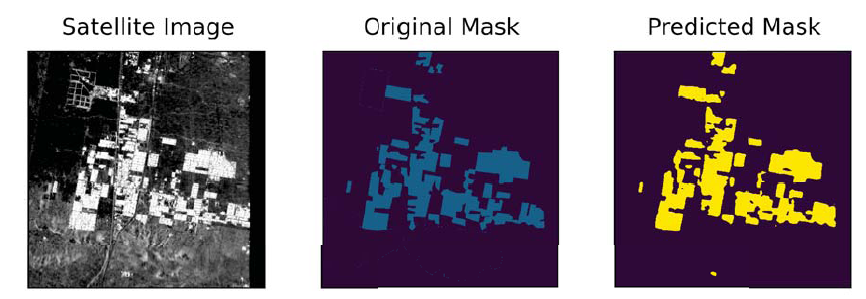
\includegraphics[width=\textwidth]{pspnet.PNG}
	\includegraphics[width=\textwidth]{pspnet-vgg19.png}

 \caption{\label{fig:psp}Results of prediction by PSPNet with VGG-19 backbone.}
\end{figure}
\begin{figure}[!htbp]
	\centering
	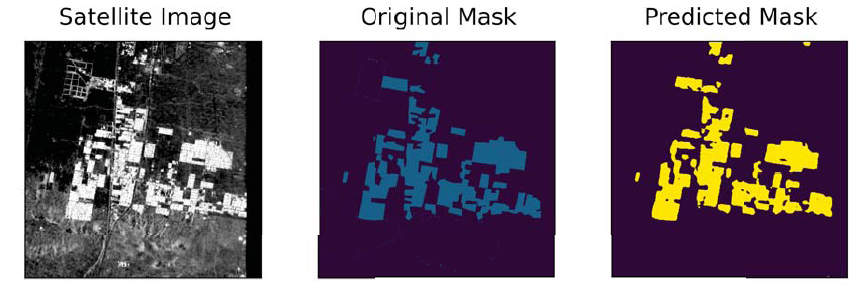
\includegraphics[width=\textwidth]{mrcnn.PNG}
 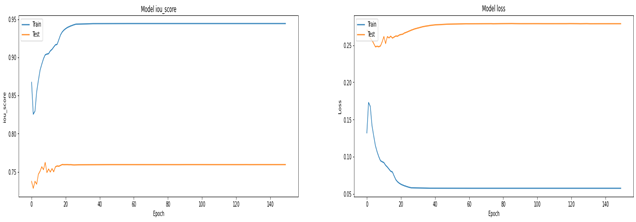
\includegraphics[width=\textwidth]{mrcnn-resnet101.png}
	\caption{\label{fig:mrcnn}Results of prediction by MRCNN with ResNext-101 backbone.}
\end{figure}
The prediction masks with our proposed technique are given in Figure \ref{fig:fpn}, \ref{fig:psp} and \ref{fig:mrcnn}. It can be seen from Figures that the top three performing model architectures are FPN with ResNet152, M-RCNN with ResNet101, and PSPNet with VGG19. This is because as we have seen that values of considered parameters for FPN are highest with ResNet152, for M-RCNN are better with ResNet101 and for PSPNet are also best with VGG19. 
The pixel accuracy, cohen’s kappa, IoU score, AuC, Recall Precision, and F1 Score of MR-CNN with ResNet101 is better compared to other backbone networks.
Finally, we present the convergence analysis of our proposed technique. We shows the convergence of the model architectures against each considered backbone networks. The CLAHE, Gaussian Blurr and different types of augmentation like translation, Rotation, Flipping have been done. 
\begin{figure}[!htbp]
	\centering
	\includegraphics[width=\textwidth]{FPN resnet50.png}
     \caption{FPN with resnet50 backbone}
 \includegraphics[width=\textwidth]{FPN resnet152.png}
 \caption{FPN with resnet152 backbone}
 \includegraphics[width=\textwidth]{FPN VGG19.png}
 \caption{FPN with VGG192 backbone}
 \end{figure}
Prediction by FPN With Resnet50, ResNet152, VGG19 as backbone FPN with ResNet152 is highest compared to all other scores. Similarly, Table 4 shows that mAP,AuC and F1 Scores for FPN with ResNet152 and VCG19 are highest respectively. Therefore, it may be concluded that the FPN gives the best accuracy among all models proposed in this paper.The high F1 score and AuC scores for the top three models confirm that the FPN architecture per-forms best among all other architectures. It gives pixel accuracy above 90%  
for three backbones, namely ResNet152, VGG-19, and ResNet50. 
\begin{figure}[!h]
	\centering
 \includegraphics[width=\textwidth]{LinkNet Inceptionv3.png}
	\caption{\label{fig:}Results of prediction by linknet with inception3 as backbone.}
 \includegraphics[width=\textwidth]{LinkNet mobilenet.png}
    \caption{Results of prediction by linknet with mobilenet as backbone.}
 \includegraphics[width=\textwidth]{LinkNet resnet152.png}
 \caption{Results of prediction by linknet with Resnet152 as backbone.}
 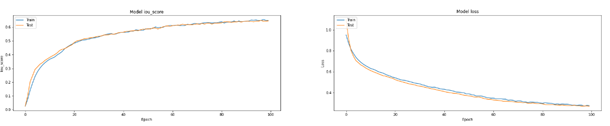
\includegraphics[width=\textwidth]{linknet-efficientnet.png}
    \caption{Results of prediction by link-net with efficient-net as backbone.}
   
\includegraphics[width=\textwidth]{LinkNet vgg19.png}
   \caption{results of prediction by linknet with VGG19 as backbone.}
   \end{figure}
The Pixel Accuracy of 91\% for LinkNet with ResNet152 is highest.The values of Recall and Precision are highest for LinkNet with ResNet50 and ResNet152 respectively.
 \begin{figure}[!h]
	\centering
	\includegraphics[width=\textwidth]{PSPNet inceptionresnetv2.png}
    \caption{Results of prediction by Pspnet with inception2 as backbone.}
    \includegraphics[width=\textwidth]{PSPNet mobilenet.png}
    \caption{Results of prediction by Pspnet with mobilenet as backbone.}
 \includegraphics[width=\textwidth]{PSPNet resnet50.png}
	\caption{\label{fig:}Results of prediction by pspnet  with Resnet50 as backbone.}
 \includegraphics[width=\textwidth]{PSPNet resnet152.png}
   \caption{Results of prediction by pspnet with resnet152 as backbone.}
% \includegraphics[width=\textwidth]{}
%    \caption{results of prediction by PSPNet with VGG19 as backbone.}
%  \end{figure}
The Pixel Accuracy with ResNet50 and Cohen’s Kappa Score and IoU Score with VGG19 for PSP-Net are better compared to other two backbone networks. The values of AuC with ResNet50, Recall with ResNet152 Precision and F1 Score with ResNet50 are best. It can specifically be inferred about PSPNet that the PSPNet architecture performs well with VGG-19, ResNet50 and ResNet152 respectively as its backbone networks.
% \bgroup
% \def\arraystretch{1.1}%
% \begin{table}[]
% \centering
% \caption{Convergence Analysis}
% \label{TabConv}
% \begin{tabular}{|c|c|c|}
% \hline
% \textbf{Model Architecture} &
%   \textbf{Backbone Network} &
%   \textbf{Time(in ms)}   \\ \hline
%                                  & \textbf{ResNet152} & xx \\ \cline{2-3}
%                                  & \textbf{ResNet101}   & xx  \\ \cline{2-3}
%                                  & \textbf{ResNet50}   & xx  \\ \cline{2-3}
% \multirow{-4}{*}{\textbf{FPN}}   & \textbf{VGG-19}     & xx  \\ \hline
%                                 & \textbf{ResNet152}   & xx  \\ \cline{2-3}
%                                  & \textbf{ResNet101} & xx  \\ \cline{2-3}
%                                  & \textbf{ResNet50}   & xx   \\ \cline{2-3}
% \multirow{-4}{*}{\textbf{MR-CNN}} & \textbf{VGG-19}     & xx   \\ \hline
%                                   &  \textbf{ResNet152} &    xx   \\ \cline{2-3}
%                                   & \textbf{ResNet101}   & xx  \\ \cline{2-3}
%                                  & \textbf{ResNet50}   &  xx   \\ \cline{2-3}
% \multirow{-4}{*}{\textbf{PSPNet}} & \textbf{VGG-19}     & xx   \\ \hline
% {\color[HTML]{222222} }          & \textbf{ResNet152}  &  xx   \\ \cline{2-3}
%                                 & \textbf{ResNet101}   & xx  \\ \cline{2-3}
% {\color[HTML]{222222} }          &   \textbf{ResNet50} &  xx   \\ \cline{2-3}
% \multirow{-4}{*}{{\color[HTML]{222222} \textbf{LinkNet}}} & \textbf{VGG-19}     & xx   \\ \hline
% \end{tabular}
% \label{tab:results2}
% \end{table}
% \egroup
We also present a graph plotting the convergence time for all model architectures against each backbone networks in Figure 
Linknet has lowest precision so the prediction mask is omitted.
\section{Conclusion}
This paper presents an image segmentation and classification technique of urban cover areas using Polarimetric SAR (PolSAR) which works based on Deep Neural Networks (DNNs) such as PSPNet, LinkNet, FPN, and Mask-RCNN. Here, we first applied polarimetric decomposition on airborne Uninhabited Aerial Vehicle Synthetic Aperture (UAVSAR) images of urban areas and then the decomposed images are fed into DNNs for segmentation and classification. Four different experimentations are carried out using four different databases and models such as PSPNet, LinkNet, FPN, and Mask-RCNN and then results obtained from the experimentations are compared with different backbone networks such as ResNet152, ResNet101, ResNet50, and VGG19. In comparison, it is seen that the FPN model with the ResNet152 as a backbone network obtained the best results on considered performance metrics such as mean Average Precision Score (mAP) and pixel accuracy. Specifically, it achieves the pixel accuracy of 90.9\% and the mAP score of 0.823 and outperforms other Deep Learning models. In the future, the authors would like to explore for integrating the proposed technique for change detection and classification of multi-class objects in the domain of image processing. 
% \bibliography{references}   % bibliography data in report.bib
\bibliography{report.bib}   % bibliography data in report.bib
% \bibliography{utube.bib}   % bibliography data in report.bib
\bibliographystyle{spiejour}   % makes bibtex use spiejour.bst
% \bibliographystyle{plain}   % makes bibtex use spiejour.bst
%\bibliographystyle{authordate1}

\end{spacing}
\end{document} 